%****************************************************************************************
%****************************************************************************************
\documentclass[12pt]{DTI}
\usepackage{graphicx}
\usepackage{gensymb}
\usepackage{enumitem}
\usepackage{listing}
\usepackage[titletoc]{appendix}
%\usepackage{epsfig}
%\usepackage[latin1]{inputenc} %nel caso di Windows;
%\usepackage[utf8x]{inputenc} % nel caso di Linux (richiede il pacchetto unicode);
\usepackage[english]{babel}
%\usepackage[italian]{babel}
\usepackage{booktabs}
\usepackage{float,lscape}
\usepackage{verbatim}
\usepackage{url}
\usepackage{tikz}
%\usepackage{tikz-qtree}
\usepackage{color}
\usepackage{listings}
\usepackage{fancybox}
%\usepackage{flowchart}
\usepackage{adjustbox}



\usepackage{draftwatermark}  %enable only when using as DRAFT
\SetWatermarkText{DRAFT} % set watermark in the whole document
\SetWatermarkScale{4}
\SetWatermarkLightness{0.93}

\newcommand{\return}{%
\raisebox{1.2pt}{\setlength{\fboxsep}{2pt}\ovalbox{$\hookleftarrow$}}}
\let\CR\return
\let\RET\return

\usepackage{hyperref}	% Reference the contents and figures
\usepackage{mathtools}
%\usepackage{fixltx2e}



\lstset{ %
	language=C++,                % choose the language of the code
	basicstyle=\footnotesize,       % the size of the fonts that are used for the code
	numbers=left,                   % where to put the line-numbers
	numberstyle=\footnotesize,      % the size of the fonts that are used for the line-numbers
	stepnumber=1,                   % the step between two line-numbers. If it is 1 each line will be numbered
	numbersep=5pt,                  % how far the line-numbers are from the code
	backgroundcolor=\color{white},  % choose the background color. You must add \usepackage{color}
	showspaces=false,               % show spaces adding particular underscores
	showstringspaces=false,         % underline spaces within strings
	showtabs=false,                 % show tabs within strings adding particular underscores
	frame=single,           % adds a frame around the code
	tabsize=2,          % sets default tabsize to 2 spaces
	captionpos=b,           % sets the caption-position to bottom
	breaklines=true,        % sets automatic line breaking
	breakatwhitespace=false,    % sets if automatic breaks should only happen at whitespace
	escapeinside={\%*}{*)},          % if you want to add a comment within your code
	keywordstyle=\color{blue},
	stringstyle=\color{red},
	commentstyle=\color{green},
	morecomment=[l][\color{magenta}]{\#}
}
\newcommand{\mytilde}{\raise.17ex\hbox{$\scriptstyle\mathtt{\sim}$}}
\newcommand{\myXOR}{$\wedge\:$}


\usetikzlibrary{%
  arrows,%
  shapes.misc,% wg. rounded rectangle
  shapes.arrows,%
  chains,%
  matrix,%
  positioning,% wg. " of "
  scopes,%
  decorations.pathmorphing,% /pgf/decoration/random steps | erste Graphik
  shadows%
}

\usetikzlibrary{shadows,trees}
\usetikzlibrary{trees}

\usetikzlibrary{positioning}
\usetikzlibrary{shapes,arrows}
\headtitle{Intern Practices}
\footauthor{Armando Rivero SUPSI--DTI, CH-6928 Manno}


\newcommand{\forceindent}{\parindent=2em\indent\parindent=0pt\relax} %remove indentation

%****************************************************************************************
%****************************************************************************************

%========================================================================================
\begin{document}



\tikzset{
  nonterminal/.style={
    % The shape:
    rectangle,
    % The size:
    minimum size=6mm,
    % The border:
    very thick,
    draw=red!50!black!50,         % 50% red and 50% black,
                                  % and that mixed with 50% white
    % The filling:
    top color=white,              % a shading that is white at the top...
    bottom color=red!50!black!20, % and something else at the bottom
    % Font
    font=\itshape
  },
	mykeyword/.style={
    % The shape:
    rounded rectangle,
    % The size:
    minimum size=6mm,
    % The border:
    very thick,
    draw=red!50!black!50,         % 50% red and 50% black,
                                  % and that mixed with 50% white
    % The filling:
    top color=white,              % a shading that is white at the top...
    bottom color=red!50!black!20, % and something else at the bottom
    % Font
    font=\itshape
  },
  terminal/.style={
    % The shape:
    rectangle, rounded corners, 
    minimum size=6mm,
    % The rest
    very thick,draw=black!50,
    top color=white,bottom color=black!20,
  %font=\ttfamily
	},
	round2/.style={
    % The shape:
    circle,
    minimum size=6mm,
    % The rest
    very thick,draw=black!50,
    top color=white,bottom color=black!20,
  %font=\ttfamily
	},
  skip loop/.style={to path={-- ++(0,#1) -| (\tikztotarget)}}
}


\date{02.04.2015}

\author{A. Rivero - S. Guatieri}
\title{%
Intern Experiments
\\[5mm]
Using a Stepper Motor
\\[3mm]
{\small Hardware: Arduino + Motor Driver + External Electronics}
}
\maketitle
~\vspace{5mm}
\begin{center}
{\sf Revision}
\end{center}
\vspace{10mm}
\begin{tabular}{|p{15mm}p{25mm}p{20mm}p{73mm}}
{\sf Date} &{\sf Author} &{\sf State} &{\sf Reason}\\\hline
02.04.15 & A. Rivero & V1.0 &...................\\\hline

\end{tabular}



%\addtocontents{toc}{~\hfill\textbf{Page}\par}
%\addcontentsline{toc}{chapter}{Contents}
%\setcounter{tocdepth}{4}		%set the levels of TOC
%\setcounter{secnumdepth}{4} 	%set the enumeration of TOC
\tableofcontents
%\newpage

\forceindent %this command is defined in "Gridsense_SPEC_ISEA_2014nov.tex" file

% alcuni oggetti copia incolla
% \`{e}
% \newline

% \begin{itemize}
%\item Logiche programmabili
%\item Pin o nodi
%\item Set
%\item Costanti
%\item Macro
%\item Segnali di entrata e di uscita
%\end{itemize}

%Define block styles
 % Modelli per flow chart
 \tikzstyle{decision} = [diamond, draw, fill=blue!20, text width=4.5em, text badly centered, node distance=3cm, inner sep=0pt]
\tikzstyle{block} = [rectangle, draw, fill=blue!20, text width=5em, text centered, rounded corners, minimum height=4em]
 \tikzstyle{line} = [draw, -latex']
 \tikzstyle{cloud} = [draw, ellipse,fill=red!20, node distance=3cm, minimum height=2em]
 % Modelli per statement di C
 \tikzstyle{mandatory_block} = [rectangle, draw, top color=white, bottom color=blue!25, 
    text width=6em, text centered, rounded corners, drop shadow, minimum height=2em]
 \tikzstyle{optional_block} = [rectangle, draw, top color=white, bottom color=red!25,
    text width=6em, text centered, rounded corners, drop shadow, minimum height=2em]
 \tikzstyle{round}=[circle, thin, draw, fill=red!20, drop shadow, minimum size=2em,inner sep=0pt]
\tikzstyle{round1}=[circle, thin, drop shadow, minimum size=0em,inner sep=0pt]



%+++++++++++++++++++++++++++++++++++++++++++++++++++++++++++++++++++++++++++++++++++++++++
%-----------------------------------------------------------------------------------------
\chapter*{Introduction}
\label{chap: Introduction}
This document describes the Stepper Motor control using Arduino and external electronics.

%\begin{figure}[H]
%\begin{center}
%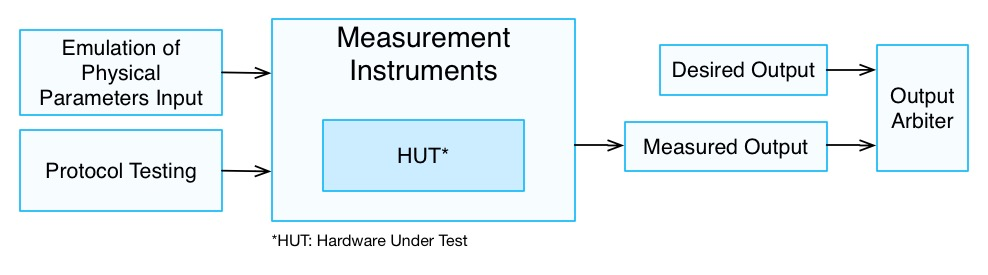
\includegraphics[scale=0.45]{immagini/Testing_Gridsense_TestSystem}
% \caption{Testing System} 
% \label{fig: Testing_Gridsense_TestSystem}
%\end{center}
%\end{figure}



\begin{enumerate}
  \item \textbf{Learn what is a stepper motor:}  (half day)
  	\subitem Student must do a small research of what is a stepper motor.
  	\subitem description of the kinds of steppers (Unipolar - Bipolar).
  \item \textbf{Learn how to use a stepper motor:} (half day)
  	\subitem Student must make a small research of how to control the two kind’s of motors and learn the sequences for each stepper.
  	\subitem Student must identify the HW needed to connect the Stepper to the Arduino. (use of LM293/LM293D)
  \item \textbf{Programming the sequence using Arduino:} (one day)
  	\subitem Using PINx of the Arduino's API
  		\subsubitem Stepper in clockwise way direction
  		\subsubitem Stepper in counter clockwise way direction
  		\subsubitem Stepper in both directions
  	\subitem Using the PORTx of the microcontroller
  		\subsubitem Stepper in clockwise way direction
  		\subsubitem Stepper in counter clockwise way direction
  		\subsubitem Stepper in both directions
  \item \textbf{Optimise the program Part 1} (one day)
	\subitem Understand the use of push buttons using Arduino
		\subsubitem Identify the bouncing effect
		\subsubitem solve the problem using "anti-bouncing" techniques
  	\subitem Add the use of push buttons to define the direction of the stepper motor (left and right).
  	\subitem Add the use of push buttons to set the velocity of the stepper motor
  \item \textbf{Optimise the program Part 2} (one day)
  	\subitem Introduce sensors to identify the position of the motor.
  	\subitem \textcolor{red}{MORE IDEAS TO ADD HERE}


\end{enumerate}




\end{document}
%========================================================================================




